
%{{第四十四回}}{第四十四回}}

\chapter{变生不测凤姐泼醋\hspace{.5em}喜出望外平儿理妆}

{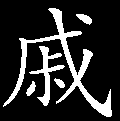
\includegraphics[width=3mm]{../Images/00005}  \kaishu 云雨谁家院,飘来花自奇。莺莺燕燕斗芳菲,枝枝因风滴玉露,正春时。}

话说众人看演《荆钗记》,宝玉和姐妹一处坐着。林黛玉因看到《男祭》这一出上,便和宝钗说道:“这王十朋也不通的很,不管在那里祭一祭罢了,必定跑到江边子上来作什么!俗语说‘睹物思人’,天下的水总归一源,不拘那里的水舀一碗看着哭去,也就尽情了。”宝钗不答。宝玉回头要热酒敬凤姐儿。

原来贾母说今日不比往日,定要叫凤姐痛乐一日。本来自己懒待坐席,只在里间屋里榻上歪着和薛姨妈看戏,随心爱吃的拣几样放在小几上,随意吃着说话儿;将自己两桌席面赏那没有席面的大小丫头并那应差听差的妇人等,命他们在窗外廊檐下也只管坐着随意吃喝,不必拘礼。王夫人和邢夫人在地下高桌上坐着,外面几席是他姊妹们坐。

贾母不时吩咐尤氏等:“让凤丫头坐在上面,你们好生替我待东,难为他一年到头辛苦。”尤氏答应了,又笑回说道:“他坐不惯首席,坐在上头横不是竖不是的,酒也不肯吃。”贾母听了,笑道:“你不会,等我亲自让他去。”凤姐儿忙也进来笑说:“老祖宗别信他们的话,我吃了好几钟了。”贾母笑着,命尤氏:“快拉他出去,按在椅子上,你们都轮流敬他。他再不吃,我当真的就亲自去了。”尤氏听说,忙笑着又拉他出来坐下,命人拿了台盏斟了酒,笑道:“一年到头难为你孝顺老太太、太太和我。我今儿没什么疼你的,亲自斟杯酒,乖乖儿的在我手里喝一口。”凤姐儿笑道:“你要安心孝敬我,跪下我就喝。”尤氏笑道:“说的你不知是谁!我告诉你说,好容易今儿这一遭,过了后儿,知道还得像今儿这样不得了?趁着尽力灌丧两钟罢。”{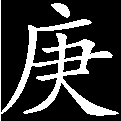
\includegraphics[width=3mm]{../Images/00004}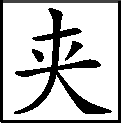
\includegraphics[width=3mm]{../Images/00012}\footnotesize \kaishu 闲闲一戏语,伏下后文,令人可伤。所谓“盛筵难再”。}凤姐儿见推不过,只得喝了两钟。

接着众姊妹也来,凤姐也只得每人的喝一口。赖大妈妈见贾母尚这等高兴,也少不得来凑趣儿,领着些嬷嬷们也来敬酒。凤姐儿也难推脱,只得喝了两口。鸳鸯等也来敬,凤姐儿真不能了,忙央告道:“好姐姐们,饶了我罢,我明儿再喝罢。”鸳鸯笑道:“真个的,我们是没脸的了?就是我们在太太跟前,太太还赏个脸儿呢。往常倒有些体面,今儿当着这些人,倒拿起主子的款儿来了。我原不该来。不喝,我们就走。”说着真个回去了。凤姐儿忙赶上拉住,笑道:“好姐姐,我喝就是了。”说着拿过酒来,满满的斟了一杯喝干。鸳鸯方笑了散去,然后又入席。

凤姐儿自觉酒沉了,心里突突的似往上撞,要往家去歇歇,只见那耍百戏的上来,便和尤氏说:“预备赏钱,我要洗洗脸去。”尤氏点头。凤姐儿瞅人不防,便出了席,往房门后檐下走来。平儿留心,也忙跟了来,凤姐儿便扶着他。才至穿廊下,只见他房里的一个小丫头正在那里站着,见他两个来了,回身就跑。凤姐儿便疑心忙叫。那丫头先只装听不见,无奈后面连平儿也叫,只得回来。

凤姐儿越发起了疑心,忙和平儿进了穿堂,叫那小丫头子也进来,把槅扇关了,凤姐儿坐在小院子的台阶上,命那丫头子跪了,喝命平儿:“叫两个二门上的小厮来,拿绳子鞭子,把那眼睛里没主子的小蹄子打烂了!”那小丫头子已经唬的魂飞魄散,哭着只管碰头求饶。凤姐儿问道:“我又不是鬼,你见了我,不说规规矩矩站住,怎么倒往前跑?”小丫头子哭道:“我原没看见奶奶来。我又记挂着房里无人,所以跑了。”凤姐儿道:“房里既没人,谁叫你来的?你便没看见我,我和平儿在后头扯着脖子叫了你十来声,越叫越跑。离的又不远,你聋了不成?你还和我强嘴!”说着便扬手一掌打在脸上,打的那小丫头一栽;这边脸上又一下,登时小丫头子两腮紫胀起来。平儿忙劝:“奶奶仔细手疼。”凤姐便说:“你再打着问他跑什么。他再不说,把嘴撕烂了他的!”那小丫头子先还强嘴,后来听见凤姐儿要烧了红烙铁来烙嘴,方哭道:“二爷在家里,打发我来这里瞧着奶奶的,若见奶奶散了,先叫我送信儿去的。不承望奶奶这会子就来了。”

凤姐儿见话中有文章,便又问道:“叫你瞧着我作什么?难道怕我家去不成?必有别的原故,快告诉我,我从此以后疼你。你若不细说,立刻拿刀子来割你的肉。”说着,回头向头上拔下一根簪子来,向那丫头嘴上乱戳,唬的那丫头一行躲,一行哭求道:“我告诉奶奶,可别说我说的。”平儿一旁劝,一面催他,叫他快说。丫头便说道:“二爷也是才来房里的,睡了一会醒了,打发人来瞧瞧奶奶,说才坐席,还得好一会才来呢。二爷就开了箱子,拿了两块银子,还有两根簪子,两匹缎子,叫我悄悄的送与鲍二的老婆去,叫他进来。他收了东西就往咱们屋里来了。二爷叫我来瞧着奶奶,底下的事我就不知道了。”

凤姐听了,已气的浑身发软,忙立起来一径来家。刚至院门,只见又有一个小丫头在门前探头儿,一见了凤姐,也缩头就跑。{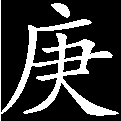
\includegraphics[width=3mm]{../Images/00004}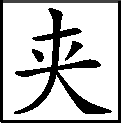
\includegraphics[width=3mm]{../Images/00012}\footnotesize \kaishu 如见其形。}凤姐儿提着名字喝住。那丫头本来伶俐,见躲不过了,越性跑了出来,笑道:“我正要告诉奶奶去呢,可巧奶奶来了。”凤姐儿道:“告诉我什么?”那小丫头便说二爷在家这般如此如此,将方才的话也说了一遍。凤姐啐道:“你早作什么了?这会子我看见你了,你来推干净儿!”说着也扬手一下打的那丫头一个趔趄,便蹑手蹑脚的走至窗前,往里听时,只听里头说笑。那妇人笑道:“多早晚你那阎王老婆死了就好了。”贾琏道:“他死了,再娶一个也是这样,又怎么样呢?”那妇人道:“他死了,你倒是把平儿扶了正,只怕还好些。”贾琏道:“如今连平儿他也不叫我沾一沾了。平儿也是一肚子委曲不敢说。我命里怎么就该犯了‘夜叉星’。”

凤姐听了,气的浑身乱战,又听他俩都赞平儿,便疑平儿素日背地里自然也有愤怨语了,那酒越发涌了上来,也并不忖夺,回身把平儿先打了两下,{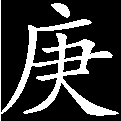
\includegraphics[width=3mm]{../Images/00004}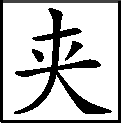
\includegraphics[width=3mm]{../Images/00012}\footnotesize \kaishu 奇极!先打平儿,可是世人想得着的?}一脚踢开门进去,也不容分说,抓着鲍二家的撕打一顿。又怕贾琏走出去,便堵着门站着骂道:“好淫妇!你偷主子汉子,还要治死主子老婆!平儿过来!你们淫妇忘八一条藤儿,多嫌着我,外面儿你哄我!”说着又把平儿打几下,打的平儿有冤无处诉,只气得干哭,骂道:“你们做这些没脸的事,好好的又拉上我做什么!”说着也把鲍二家的撕打起来。

贾琏也因吃多了酒,进来高兴,未曾作的机密,一见凤姐来了,已没了主意,又见平儿也闹起来,把酒也气上来了。凤姐儿打鲍二家的,他已又气又愧,只不好说的,今见平儿也打,便上来踢骂道:“好娼妇!你也动手打人!”平儿气怯,忙住了手,哭道:“你们背地里说话,为什么拉我呢?”凤姐见平儿怕贾琏,越发气了,又赶上来打着平儿,偏叫打鲍二家的。平儿急了,便跑出来找刀子要寻死。外面众婆子丫头忙拦住解劝。这里凤姐见平儿寻死去,便一头撞在贾琏怀里,叫道:“你们一条藤儿害我,被我听见了,倒都唬起我来。你也勒死我!”贾琏气的墙上拔出剑来,说道:“不用寻死,我也急了,一齐杀了,我偿了命,大家干净。”正闹的不开交,只见尤氏等一群人来了,说:“这是怎么说,才好好的,就闹起来。”贾琏见了人,越发“倚酒三分醉”,逞起威风来,{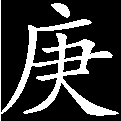
\includegraphics[width=3mm]{../Images/00004}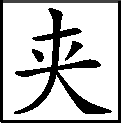
\includegraphics[width=3mm]{../Images/00012}\footnotesize \kaishu 天下小人大都如是。}故意要杀凤姐儿。凤姐儿见人来了,便不似先前那般泼了,{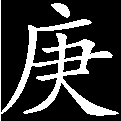
\includegraphics[width=3mm]{../Images/00004}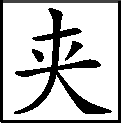
\includegraphics[width=3mm]{../Images/00012}\footnotesize \kaishu 天下奸雄、妒妇、恶妇大都如是,只是恨无阿凤之才耳。}丢下众人,便哭着往贾母那边跑。

此时戏已散出,凤姐跑到贾母跟前,爬在贾母怀里,只说:“老祖宗救我!琏二爷要杀我呢!”{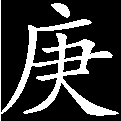
\includegraphics[width=3mm]{../Images/00004}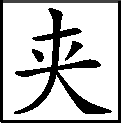
\includegraphics[width=3mm]{../Images/00012}\footnotesize \kaishu 瞧他称呼。}贾母、邢夫人、王夫人等忙问怎么了。凤姐儿哭道:“我才家去换衣裳,不防琏二爷在家和人说话,我只当是有客来了,唬得我不敢进去。在窗户外头听了一听,原来是和鲍二家的媳妇商议,说我利害,要拿毒药给我吃了治死我,把平儿扶了正。我原气了,又不敢和他吵,原打了平儿两下,问他为什么要害我。他臊了,就要杀我。”贾母等听了,都信以为真,说:“这还了得!快拿了那下流种子来!”一语未完,只见贾琏拿着剑赶来,后面许多人跟着。贾琏明仗着贾母素昔疼他们,连母亲婶母也无碍,故逞强闹了来。邢夫人王夫人见了,气的忙拦住骂道:“这下流种子!你越发反了,老太太在这里呢!”贾琏乜斜着眼,道:“都是老太太惯的他,他才这样,连我也骂起来了!”邢夫人气的夺下剑来,只管喝他“快出去!”那贾琏撒娇撒痴,涎言涎语的还只乱说。贾母气的说道:“我知道你也不把我们放在眼里,叫人把他老子叫来!”贾琏听见这话,方趔趄着脚儿出去了,赌气也不往家去,便往外书房来。

这里邢夫人王夫人也说凤姐儿。贾母笑道:“什么要紧的事!小孩子们年轻,馋嘴猫儿似的,那里保得住不这么着。从小儿世人都打这么过的。都是我的不是,他多吃了两口酒,又吃起醋来。”说的众人都笑了。贾母又道:“你放心,等明儿我叫他来替你赔不是。你今儿别要过去臊着他。”因又骂:“平儿那蹄子,素日我倒看他好,怎么暗地里这么坏。”尤氏等笑道:“平儿没有不是,是凤丫头拿着人家出气。两口子不好对打,都拿着平儿煞性子。平儿委曲的什么似的呢,老太太还骂人家。”贾母道:“原来这样,我说那孩子倒不像那狐媚魇道的。既这么着,可怜见的,白受他们的气。”因叫琥珀来:“你出去告诉平儿,就说我的话:我知道他受了委曲,明儿我叫凤姐儿替他赔不是。今儿是他主子的好日子,不许他胡闹。”

原来平儿早被李纨拉入大观园去了。{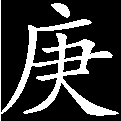
\includegraphics[width=3mm]{../Images/00004}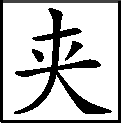
\includegraphics[width=3mm]{../Images/00012}\footnotesize \kaishu 可知吃蟹一回非闲文也。}平儿哭得哽咽难{(抬)}{[}抑{]}。宝钗劝道:“你是个明白人,{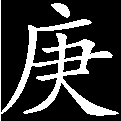
\includegraphics[width=3mm]{../Images/00004}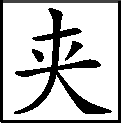
\includegraphics[width=3mm]{../Images/00012}\footnotesize \kaishu 必用宝钗评出,方是身份。}素日凤丫头何等待你,今儿不过他多吃一口酒。他可不拿你出气,难道倒拿别人出气不成?别人又笑话他吃醉了。你只管这会子委曲,素日你的好处,岂不都是假的了?”正说着,只见琥珀走来,说了贾母的话。平儿自觉面上有了光辉,方才渐渐的好了,也不往前头来。宝钗等歇息了一回,方来看贾母凤姐。

宝玉便让平儿到怡红院中来。袭人忙接着,笑道:“我先原要让你的,只因大奶奶和姑娘们都让你,我就不好让的了。”平儿也陪笑说:“多谢。”因又说道:“好好儿的从那里说起,无缘无故白受了一场气。”袭人笑道:“二奶奶素日待你好,这不过是一时气急了。”平儿道:“二奶奶倒没说的,只是那淫妇治的我,他又偏拿我凑趣,况还有我们那糊涂爷倒打我。”说着便又委曲,禁不住落泪。宝玉忙劝道:“好姐姐,别伤心,我替他两个赔不是罢。”平儿笑道:“与你什么相干?”宝玉笑道:“我们弟兄姊妹都一样。他们得罪了人,我替他赔个不是也是应该的。”又道:“可惜这新衣裳也沾了,这里有你花妹妹的衣裳,何不换了下来,拿些烧酒喷了熨一熨。把头也另梳一梳,洗洗脸。”一面说,一面便吩咐了小丫头子们舀洗脸水,烧熨斗来。

平儿素习只闻人说宝玉专能和女孩儿们接交;宝玉素日因平儿是贾琏的爱妾,又是凤姐儿的心腹,故不肯和他厮近,因不能尽心,也常为恨事。平儿今见他这般,心中也暗暗的敁敠:果然话不虚传,色色想的周到。又见袭人特特的开了箱子,拿出两件不大穿的衣裳来与他换,便赶忙的脱下自己的衣服,忙去洗了脸。宝玉一旁笑劝道:“姐姐还该擦上些脂粉,不然倒像是和凤姐姐赌气子似的。况且又是他的好日子,而且老太太又打发了人来安慰你。”平儿听了有理,便去找粉,只不见粉。宝玉忙走至妆台前,将一个宣窑磁盒揭开,里面盛着一排十根玉簪花棒,拈了一根递与平儿。又笑向他道:“这不是铅粉,这是紫茉莉花种,研碎了兑上香料制的。”平儿倒在掌上看时,果见轻白红香,四样俱美,摊在面上也容易匀净,且能润泽肌肤,不似别的粉青重涩滞。然后看见胭脂也不是成张的,却是一个小小的白玉盒子,里面盛着一盒,如玫瑰膏子一样。宝玉笑道:“那市卖的胭脂都不干净,颜色也薄。这是上好的胭脂拧出汁子来,淘澄净了渣滓,配了花露蒸叠成的。只用细簪子挑一点儿抹在手心里,用一点水化开抹在唇上;手心里就够打颊腮了。”平儿依言妆饰,果见鲜艳异常,且又甜香满颊。宝玉又将盆内的一枝并蒂秋蕙用竹剪刀撷了下来,与他簪在鬓上。忽见李纨打发丫头来唤他,方忙忙的去了。{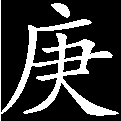
\includegraphics[width=3mm]{../Images/00004}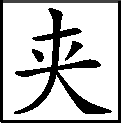
\includegraphics[width=3mm]{../Images/00012}\footnotesize \kaishu 忽使平儿在绛芸轩中梳妆,非世人想不到,宝玉亦想不到者也。作者费尽心机了。{$\diamond$}写宝玉最善闺阁中事,诸如脂粉等类,不写成别致文章,则宝玉不成宝玉矣。然要写又不便特为此费一番笔墨,故思及借人发端。然借人又无人,若袭人辈则逐日皆如此,又何必拣一日细写,似觉无味。若宝钗等又系姊妹,更不便来细搜袭人之妆奁,况也是自幼知道的了。因左想右想,须得一个又甚亲、又甚疏,又可唐突、又不可唐突,又和袭人等极亲、又和袭人等不大常处,又得袭人辈之美、又不得袭人辈之修饰一人来,方可发端。故思及平儿一人方如此,故放手细写绛芸闺中之什物也。}

宝玉因自来从未在平儿前尽过心,------且平儿又是个极聪明极清俊的上等女孩儿,比不得那起俗蠢拙物------深为恨怨。今日是金钏儿的生日,故一日不乐。{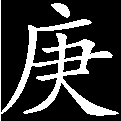
\includegraphics[width=3mm]{../Images/00004}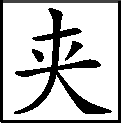
\includegraphics[width=3mm]{../Images/00012}\footnotesize \kaishu 原来为此!宝玉之私祭,玉钏之潜哀俱针对矣。然于此刻补明,又一法也。真千变万化之文,万法具备,毫无脱漏,真好书也。}不想落后闹出这件事来,竟得在平儿前稍尽片心,亦今生意中不想之乐也。因歪在床上,心内怡然自得。忽又思及贾琏惟知以淫乐悦己,并不知作养脂粉。又思平儿并无父母、兄弟姊妹,独自一人,供应贾琏夫妇二人。贾琏之俗,凤姐之威,他竟能周全妥贴,今儿还遭涂毒,想来此人薄命,比黛玉犹甚。想到此间,便又伤感起来,不觉洒然\footnote{“洒然”,诸本均同。今人或校改为“潸然”。}泪下。因见袭人等不在房内,尽力落了几点痛泪。复起身,又见方才的衣裳上喷的酒已半干,便拿熨斗熨了叠好;见他的手帕子忘去,上面犹有泪渍,又拿至脸盆中洗了晾上。又喜又悲,闷了一回,也往稻香村来,说一回闲话,掌灯后方散。

平儿就在李纨处歇了一夜,凤姐儿只跟着贾母。贾琏晚间归房,冷清清的,又不好去叫,只得胡乱睡了一夜。次日醒了,想昨日之事,大没意思,后悔不来。邢夫人记挂着昨日贾琏醉了,忙一早过来,叫了贾琏过贾母这边来。贾琏只得忍愧前来,在贾母面前跪下。贾母问他:“怎么了?”贾琏忙陪笑说:“昨儿原是吃了酒,惊了老太太的驾了,今儿来领罪。”贾母啐道:“下流东西,灌了黄汤,不说安分守己的挺尸去,倒打起老婆来了!凤丫头成日家说嘴,霸王似的一个人,昨儿唬得可怜。要不是我,你要伤了他的命,这会子怎么样?”贾琏一肚子的委屈,不敢分辩,只认不是。贾母又道:“那凤丫头和平儿还不是个美人胎子?你还不足!成日家偷鸡摸狗,脏的臭的,都拉了你屋里去。为这起淫妇打老婆,又打屋里的人,你还亏是大家子的公子出身,活打了嘴了。若你眼睛里有我,你起来,我饶了你,乖乖的替你媳妇赔个不是,拉了他家去,我就喜欢了。要不然,你只管出去,我也不敢受你的跪。”贾琏听如此说,又见凤姐儿站在那边,也不盛妆,哭的眼睛肿着,也不施脂粉,黄黄脸儿,{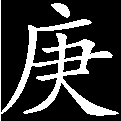
\includegraphics[width=3mm]{../Images/00004}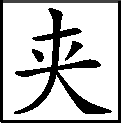
\includegraphics[width=3mm]{../Images/00012}\footnotesize \kaishu 大妙大奇之文,此一句便伏下病根了,草草看去,便可惜了作者行文苦心。}比往常更觉可怜可爱。想着:“不如赔了不是,彼此也好了,又讨老太太的喜欢了。”想毕,便笑道:“老太太的话,我不敢不依,只是越发纵了他了。”贾母笑道:“胡说!我知道他最有礼的,再不会冲撞人。他日后得罪了你,我自然也作主,叫你降伏就是了。”

贾琏听说,爬起来,便与凤姐儿作了一个揖,笑道:“原来是我的不是,二奶奶饶过我罢。”满屋里的人都笑了。贾母笑道:“凤丫头,不许恼了,再恼我就恼了。”说着,又命人去叫了平儿来,命凤姐儿和贾琏两个安慰平儿。贾琏见了平儿,越发顾不得了,{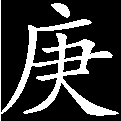
\includegraphics[width=3mm]{../Images/00004}  \kaishu 所谓“妻不如妾,妾不如偷”。}\footnote{所谓“妻不如妾,妾不如偷”,此语仅底本和甲辰本有,当是批语混入正文。}听贾母一说,便赶上来说道:“姑娘昨日受了屈了,都是我的不是。奶奶得罪了你,也是因我而起。我赔了不是不算外,还替你奶奶赔个不是。”说着,也作了一个揖,引的贾母笑了,凤姐儿也笑了。贾母又命凤姐儿来安慰他。平儿忙走上来给凤姐儿磕头,说:“奶奶的千秋,我惹了奶奶生气,是我该死。”凤姐儿正自愧悔昨日酒吃多了,不念素日之情,浮躁起来,为听了旁人的话,无故给平儿没脸。今反见他如此,又是惭愧,又是心酸,忙一把拉起来,落下泪来。平儿道:“我伏侍了奶奶这么几年,也没弹我一指甲。就是昨儿打我,我也不怨奶奶,都是那淫妇治的,怨不得奶奶生气。”说着,也滴下泪来了。{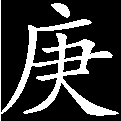
\includegraphics[width=3mm]{../Images/00004}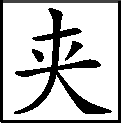
\includegraphics[width=3mm]{../Images/00012}\footnotesize \kaishu 妇人女子之情毕肖,但世之大英雄羽翼偶摧,尚按剑生悲,况阿凤与平儿哉?所谓此书真是哭成的。}贾母便命人:“将他三人送回房去。有一个再提此事,即刻来回我,我不管是谁,拿拐棍子给他一顿。”

三个人从新给贾母、邢王二位夫人磕了头。老嬷嬷答应了,送他三人回去。至房中,凤姐儿见无人,方说道:“我怎么像个阎王,又像夜叉?那淫妇咒我死,你也帮着咒。我千日不好,也有一日好。可怜我熬的连个淫妇也不如了,我还有什么脸来过这日子?”说着又哭了。{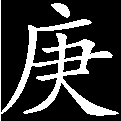
\includegraphics[width=3mm]{../Images/00004}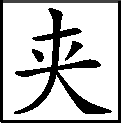
\includegraphics[width=3mm]{../Images/00012}\footnotesize \kaishu 辖治丈夫,此是首计,懦夫来看此句。}贾琏道:“你还不足?你细想想,昨儿谁的不是多?{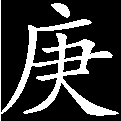
\includegraphics[width=3mm]{../Images/00004}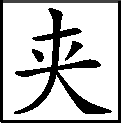
\includegraphics[width=3mm]{../Images/00012}\footnotesize \kaishu 妙!不敢自说没不是,只论多少,懦夫来看。}今儿当着人还是我跪了一跪,又赔不是,你也争足了光了。这会子还叨叨,难道还叫我替你跪下才罢?太要足了强也不是好事。”说的凤姐儿无言可对,平儿“嗤”的一声又笑了。贾琏也笑道:“又好了!真真我也没法了。”

正说着,只见一个媳妇来回说:“鲍二媳妇吊死了。”{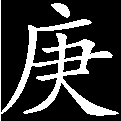
\includegraphics[width=3mm]{../Images/00004}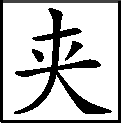
\includegraphics[width=3mm]{../Images/00012}\footnotesize \kaishu 倒也有气性,只是又是情累一个,可怜!}贾琏凤姐儿都吃了一惊。凤姐忙收了怯色,反喝道:“死了罢了,有什么大惊小怪的!”{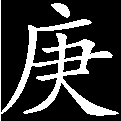
\includegraphics[width=3mm]{../Images/00004}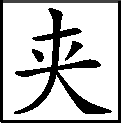
\includegraphics[width=3mm]{../Images/00012}\footnotesize \kaishu 写阿凤如此。}一时,只见林之孝家的进来悄回凤姐道:“鲍二媳妇吊死了,他娘家的亲戚要告呢。”凤姐儿笑道:{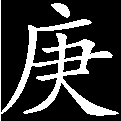
\includegraphics[width=3mm]{../Images/00004}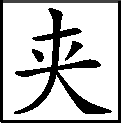
\includegraphics[width=3mm]{../Images/00012}\footnotesize \kaishu 偏于此处写阿凤笑。坏哉阿凤!}“这倒好了,我正想要打官司呢!”林之孝家的道:“我才和众人劝了他们,又威吓了一阵,又许了他几个钱,也就依了。”凤姐儿道:“我没一个钱!有钱也不给,只管叫他告去。也不许劝他,也不用震吓他,只管让他告去。告不成倒问他个‘以尸讹诈’!”{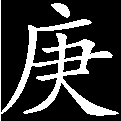
\includegraphics[width=3mm]{../Images/00004}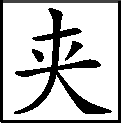
\includegraphics[width=3mm]{../Images/00012}\footnotesize \kaishu 写阿凤如此。}林之孝家的正在为难,见贾琏和他使眼色儿,心下明白,便出来等着。贾琏道:“我出去瞧瞧,看是怎么样。”凤姐儿道:“不许给他钱。”贾琏一径出来,和林之孝来商议,着人去作好作歹,许了二百两发送才罢。贾琏生恐有变,又命人去和王子腾说,将番役仵作人等叫了几名来,帮着办丧事。那些人见了如此,纵要复辨亦不敢辨,只得忍气吞声罢了。贾琏又命林之孝将那二百银子入在流年账上,分别添补开销过去。{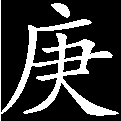
\includegraphics[width=3mm]{../Images/00004}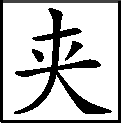
\includegraphics[width=3mm]{../Images/00012}\footnotesize \kaishu 大弊小弊,无一不到。}又梯己给鲍二些银两,安慰他说:“另日再挑个好媳妇给你。”鲍二又有体面,又有银子,有何不依,便仍然奉承贾琏,{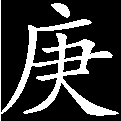
\includegraphics[width=3mm]{../Images/00004}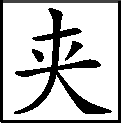
\includegraphics[width=3mm]{../Images/00012}\footnotesize \kaishu 为天下夫妻一哭。}不在话下。

里面凤姐心中虽不安,面上只管佯不理论,因房中无人,便拉平儿笑道:“我昨儿灌丧了酒了,你别愤怨,打了那里,让我瞧瞧。”平儿道:“也没打重。”只听得说,奶奶姑娘都进来了。要知端的,下回分解。

{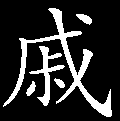
\includegraphics[width=3mm]{../Images/00005}  \kaishu 总评:富贵少年多好色,那如宝玉会风流。阎王夜叉谁曾说,死到临头身不由。}